% Datasets
% https://www.kaggle.com/manyregression/updated-wine-enthusiast-review
% https://www.kaggle.com/zynicide/wine-reviews
% https://databank.worldbank.org/reports.aspx?source=2&series=SH.ALC.PCAP.LI#
\section{Introduction}
Wine has been produced for thousands of years, with the earliest evidence of its production dating back to ancient Georgia \cite{McGovernJalabadze2017}; its importance to human culture is unquestionable, and the intricacies behind its production very vast. As well-summarized by Charles Spence, this alcoholic beverage `is a complex, culture-laden, multisensory stimulus' \cite{Spence2020}.

In an effort to better understand the current state of wine culture, and what factors affect the enjoyability of wine, a dataset containing wine reviews published by \emph{Wine Enthusiast} magazine will be explored. Throughout this work, it is important to note that \emph{Wine Enthusiast} only writes reviews for products that are rated 80 points and above, which on their scale, means wines that are \emph{acceptable}---those that can `be employed in casual, less-critical circumstances' \cite{WineMag}. % Thus, this study will aim to understand the properties of good wine.

\section{Exploration}
The two datasets combined contain all of the wine reviews published until 2020. Though the datasets have slightly different schemas, in general, each row contained the following information:
\begin{itemize}
    \setlength\itemsep{0.1em}
    \item Name of the wine
    \item Type of wine
    \item Price of the wine
    \item Vineyard where the grapes were grown
    \item Name of winery that produced the wine
    \item Country where wine was produced
    \item Other location information (province, region, and sub-region)
    \item Points given by the taster
    \item Review written by the taster
    \item Taster's name, Twitter handle, and photo URL
\end{itemize}

\subsection{Initial Research Questions}
Upon initial analysis of the attributes, the following research questions were postulated:
\begin{enumerate}
    \setlength\itemsep{0.1em}
    \item Which country's wines have been reviewed the most?
    \item Which country has the highest rated wines?
    \item Which tasters are the harshest and the kindest?
    \item Is price correlated with taste? Is pricier wine better than cheaper wine?
\end{enumerate}

\section{General Data Processing and Cleaning}
In general, not much cleaning and pre-processing was required. Firstly, the attributes not relevant to our research questions were dropped, and the schemas of the two datasets were made to be the same so that they could be joined. Continent data was also mapped to each wine from the country of production using the library \code{countrycode}; this was done because multiple visualizations require this data.

There were also a few non-ASCII characters that had to be replaced. The non breaking space character found in the taster name `Anne Krebiehl MW' was replaced with a normal white space. The special apostrophe character found in the name ``Kerin o \textquotesingle Keefe'' was replaced with an escaped apostrophe to prevent errors when displaying the taster's name in the visualizations.

\section{Visualizations}

% 11111111111
\subsection{Which country's wines have been reviewed the most?}
Initially, to answer this question, a bar chart was plotted due to its ubiquity. However, the Cleveland dot plot was instead used for the final visualization. This plot was chosen over the more common bar chart to follow Tufte's principles on the so called \emph{data-ink ratio}. As stated by Tufte, ``[a] large share of ink on a graphic should present data-information, the ink changing as the data change.'' This means that maintaining a high data-ink ratio---expressed as the formula
$$
\textrm{Data-ink ratio} = \frac{\textrm{Data-ink}}{\textrm{Total ink used}}
$$

\noindent ---is often a good rule of thumb to follow in order to produce good visualizations. Though this rule should not be strictly adhered to in all cases, it may definitely be applied to the bar chart since the area of the bars are redundant data-ink---only the position where the bar ends is required to express the data \cite{Tufte}. Another reason for choosing the dot plot was because according to Mackinlay's effectiveness ranking, position is the most effective for encoding quantitative data \cite{Mackinlay}. Meanwhile, hue was chosen to encode the continents because according to the ranking, it is the second most effective for nominal data.

\begin{figure}[h]
  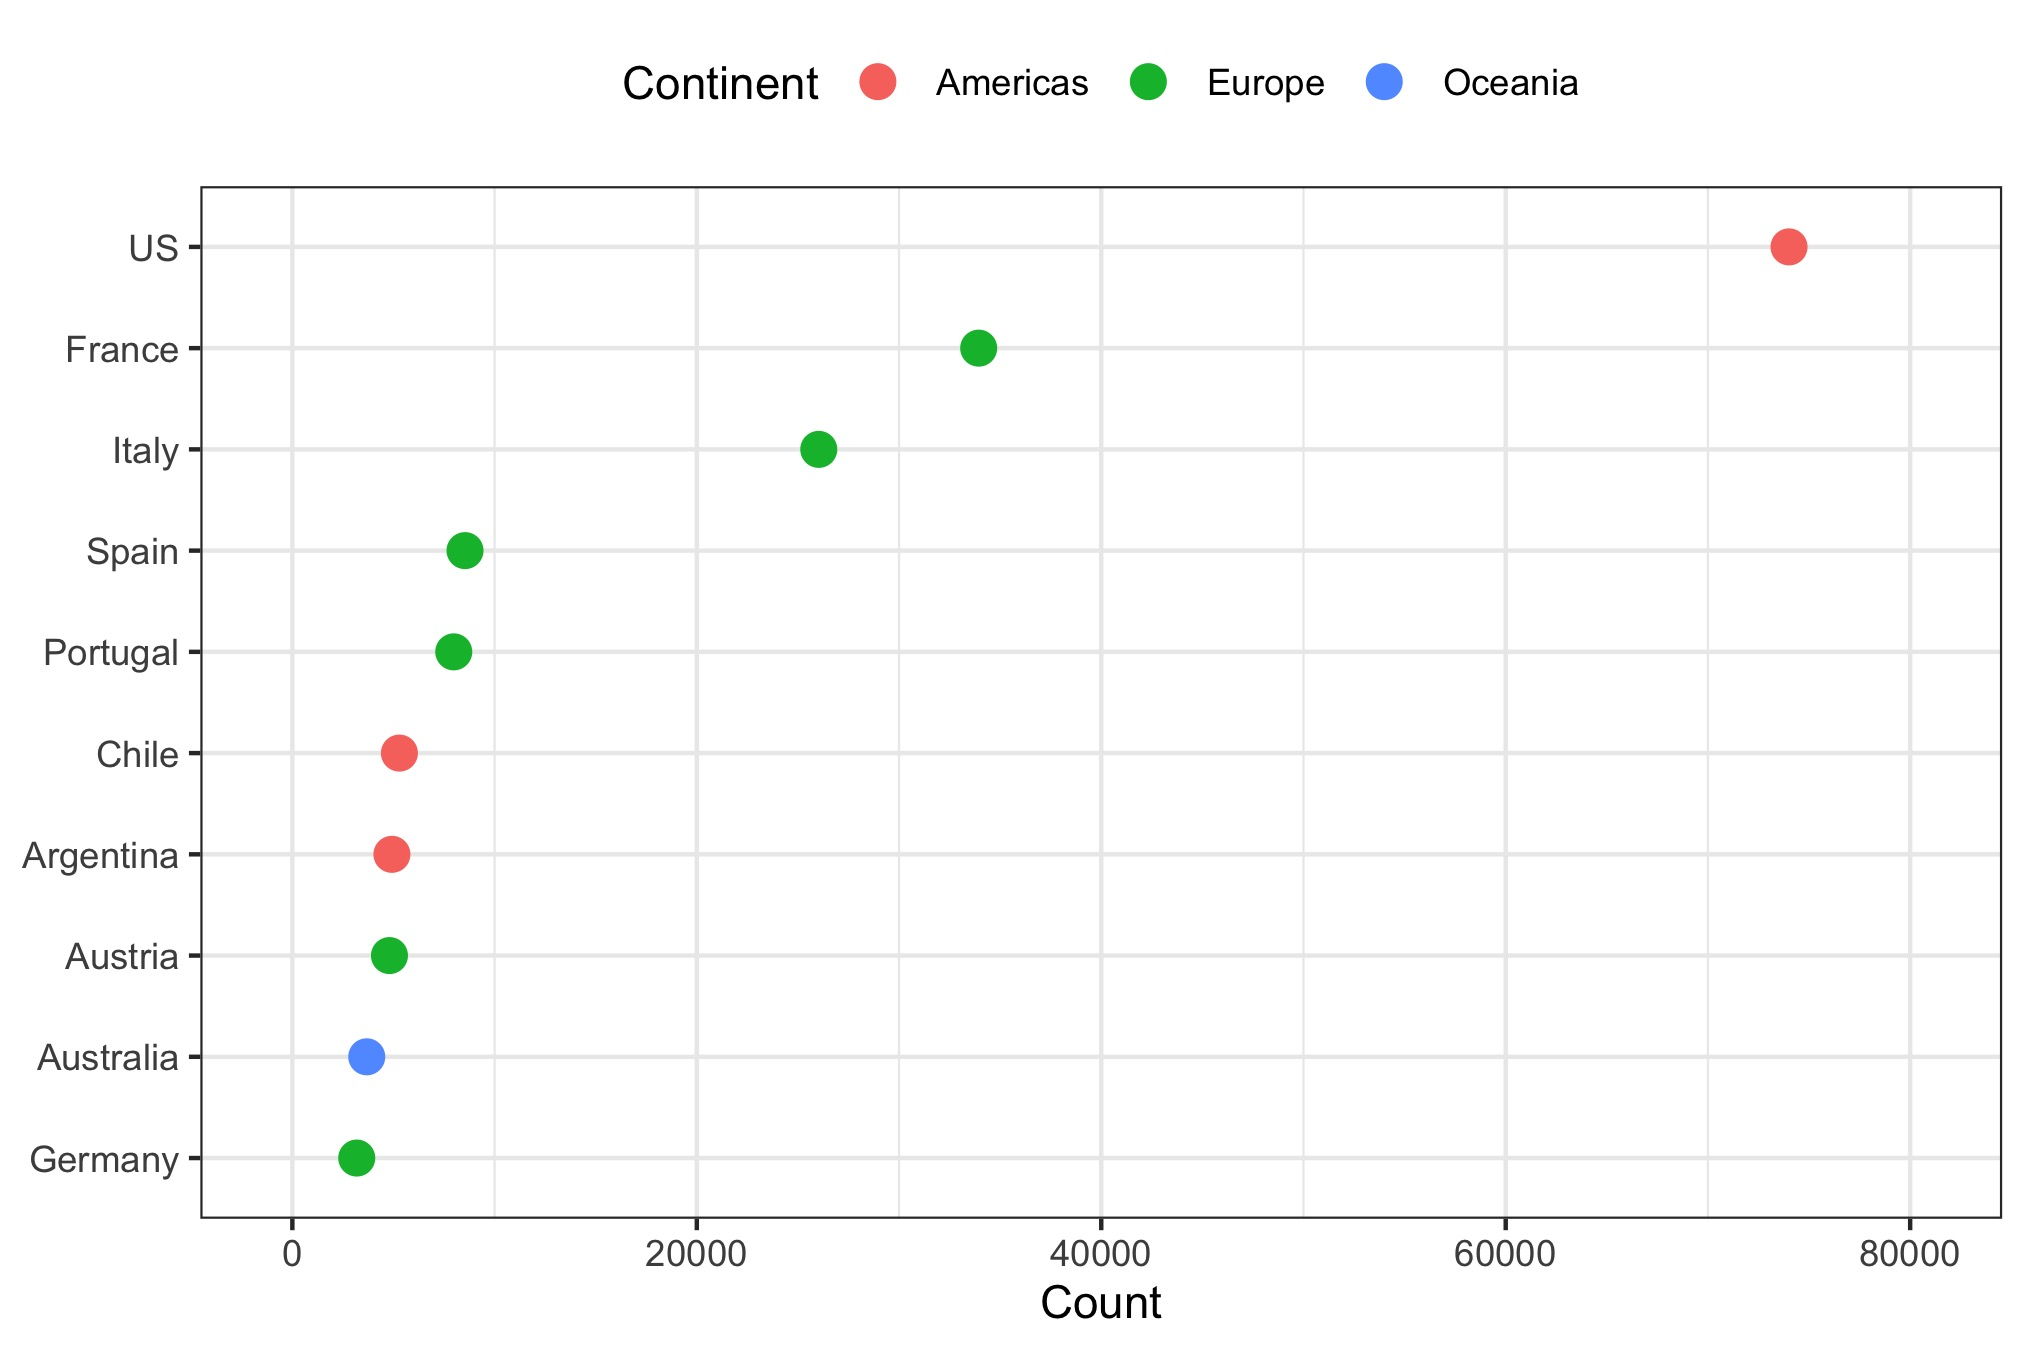
\includegraphics[width=0.95\linewidth]{1.jpg}  
  \caption{Countries by number of wine reviews}
\end{figure}

Processing of the data was done by: (1) dropping the rows without a country, (2) grouping the rows by country, (3) counting the number of reviews per country, and (4) slicing the top 10 countries by the number of reviews. While the rest of the countries could have been included, they did not provide more interesting data because they had so little reviews, and thus, their differences could not be easily understood from the plot. Furthermore, while the $x$-axis could have been scaled to better see the information for the countries with less reviews, the intention of this visualization is primarily to show clearly and concisely the difference in number of reviews per country.

As shown by figure 1, it is easy to see that a large share of wines reviewed by the magazine are from the United States even though the top three producers worldwide are Italy, France, and Spain \cite{Statista}. This is most likely the case because \emph{Wine Enthusiast} is based in the United States, and thus, has easier access to wines produced there.



To present the data in a meaningful order, the countries are displayed from high to low number of reviews using the \code{reorder()} function.

% 2222222222
\subsection{From the most reviewed countries, which has the best reviews?}
Initially, this question aimed to explore, out of all countries, which ones had the best reviews. However, after answering the previous question and discovering that the other countries had significantly less reviews (and thus, a less representative sample size), it was decided to instead only explore this question for the ten most reviewed countries. Box plots and violin plots were first experimented with, however, they were not as clear and concise as the point range plot and provided too much information that cluttered the visualization.

Processing of the data involved grouping the data by country and continent, calculating the mean and standard deviation of the points for each country, counting the number of reviews for each country, and slicing the top 10 countries by the previous counts.

\begin{figure}[h]
  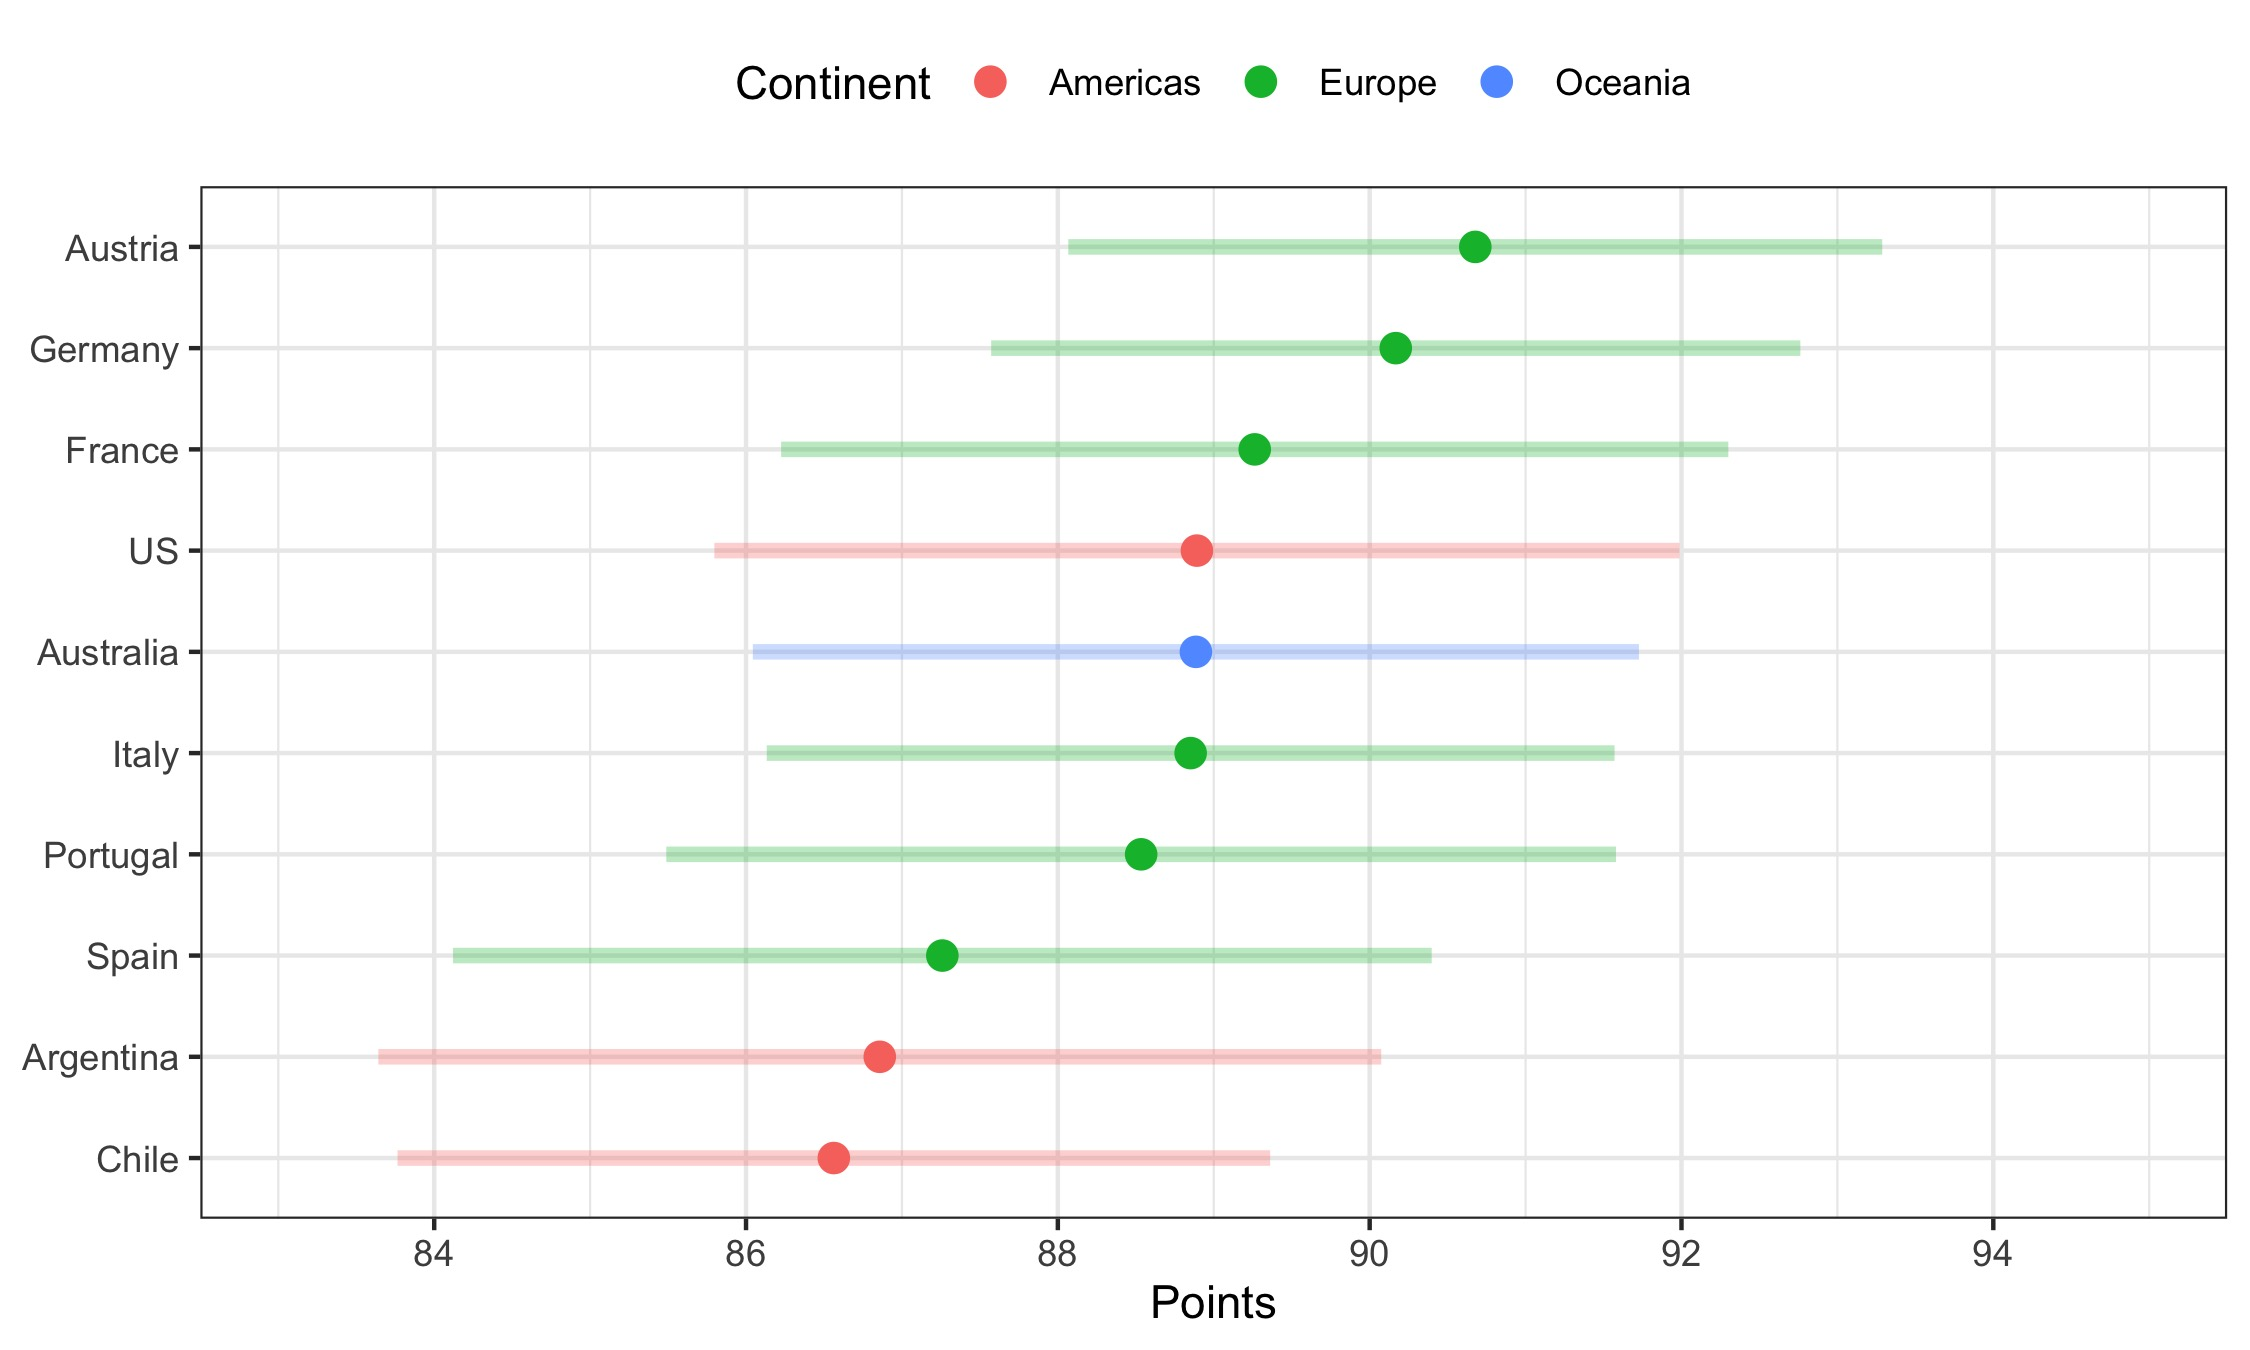
\includegraphics[width=0.95\linewidth]{2.jpg} 
  \caption{Mean and standard deviation of scoring for the 10 most reviewed countries}
\end{figure}

Similarly to the visualization for question 1, position was used to encode the means while hue was used to encode the continents. Length is used to encode the standard deviation of each mean because it is the second most effective for encoding quantitative values according to Mackinlay \cite{Mackinlay}. Additionally, the opacity of the bars was lowered to put more emphasis on the means; this was accomplished by layering a dot plot of the means on top of the point range plot and lowering the opacity of the latter because in \code{ggplot2}, it is not possible to lower only the opacity of the bars in a point range plot.

As shown by figure 2, Austria, Germany, and France had the highest mean scores while the US was only in fourth place. This however, is most likely not representative of how good each country's wines are because compared to the US, wines from other countries have significantly less reviews.

% 3333333333333
\subsection{Which tasters are the harshest and the kindest?}
The final question aims to explore the scoring of each taster. Even though the genders of the tasters were not part of the original dataset, they were collected and visualized in the plot to explore whether there is a noticeable scoring difference between the two genders.

Processing of the data involved grouping the data by taster, and calculating the mean and standard deviation of each taster's scoring. The rows without taster names were dropped. The previous result was then left joined (by taster name) with a table containing the gender of each taster.

The rationale for the selection of visual encodings was the same as the one for the previous visualization. Like in the previous visualizations, the nominal variable (taster names) was encoded to the $y$-axis for clarity, because if the $x$-axis was used, it would be harder to read the names.

\begin{figure}[h]
  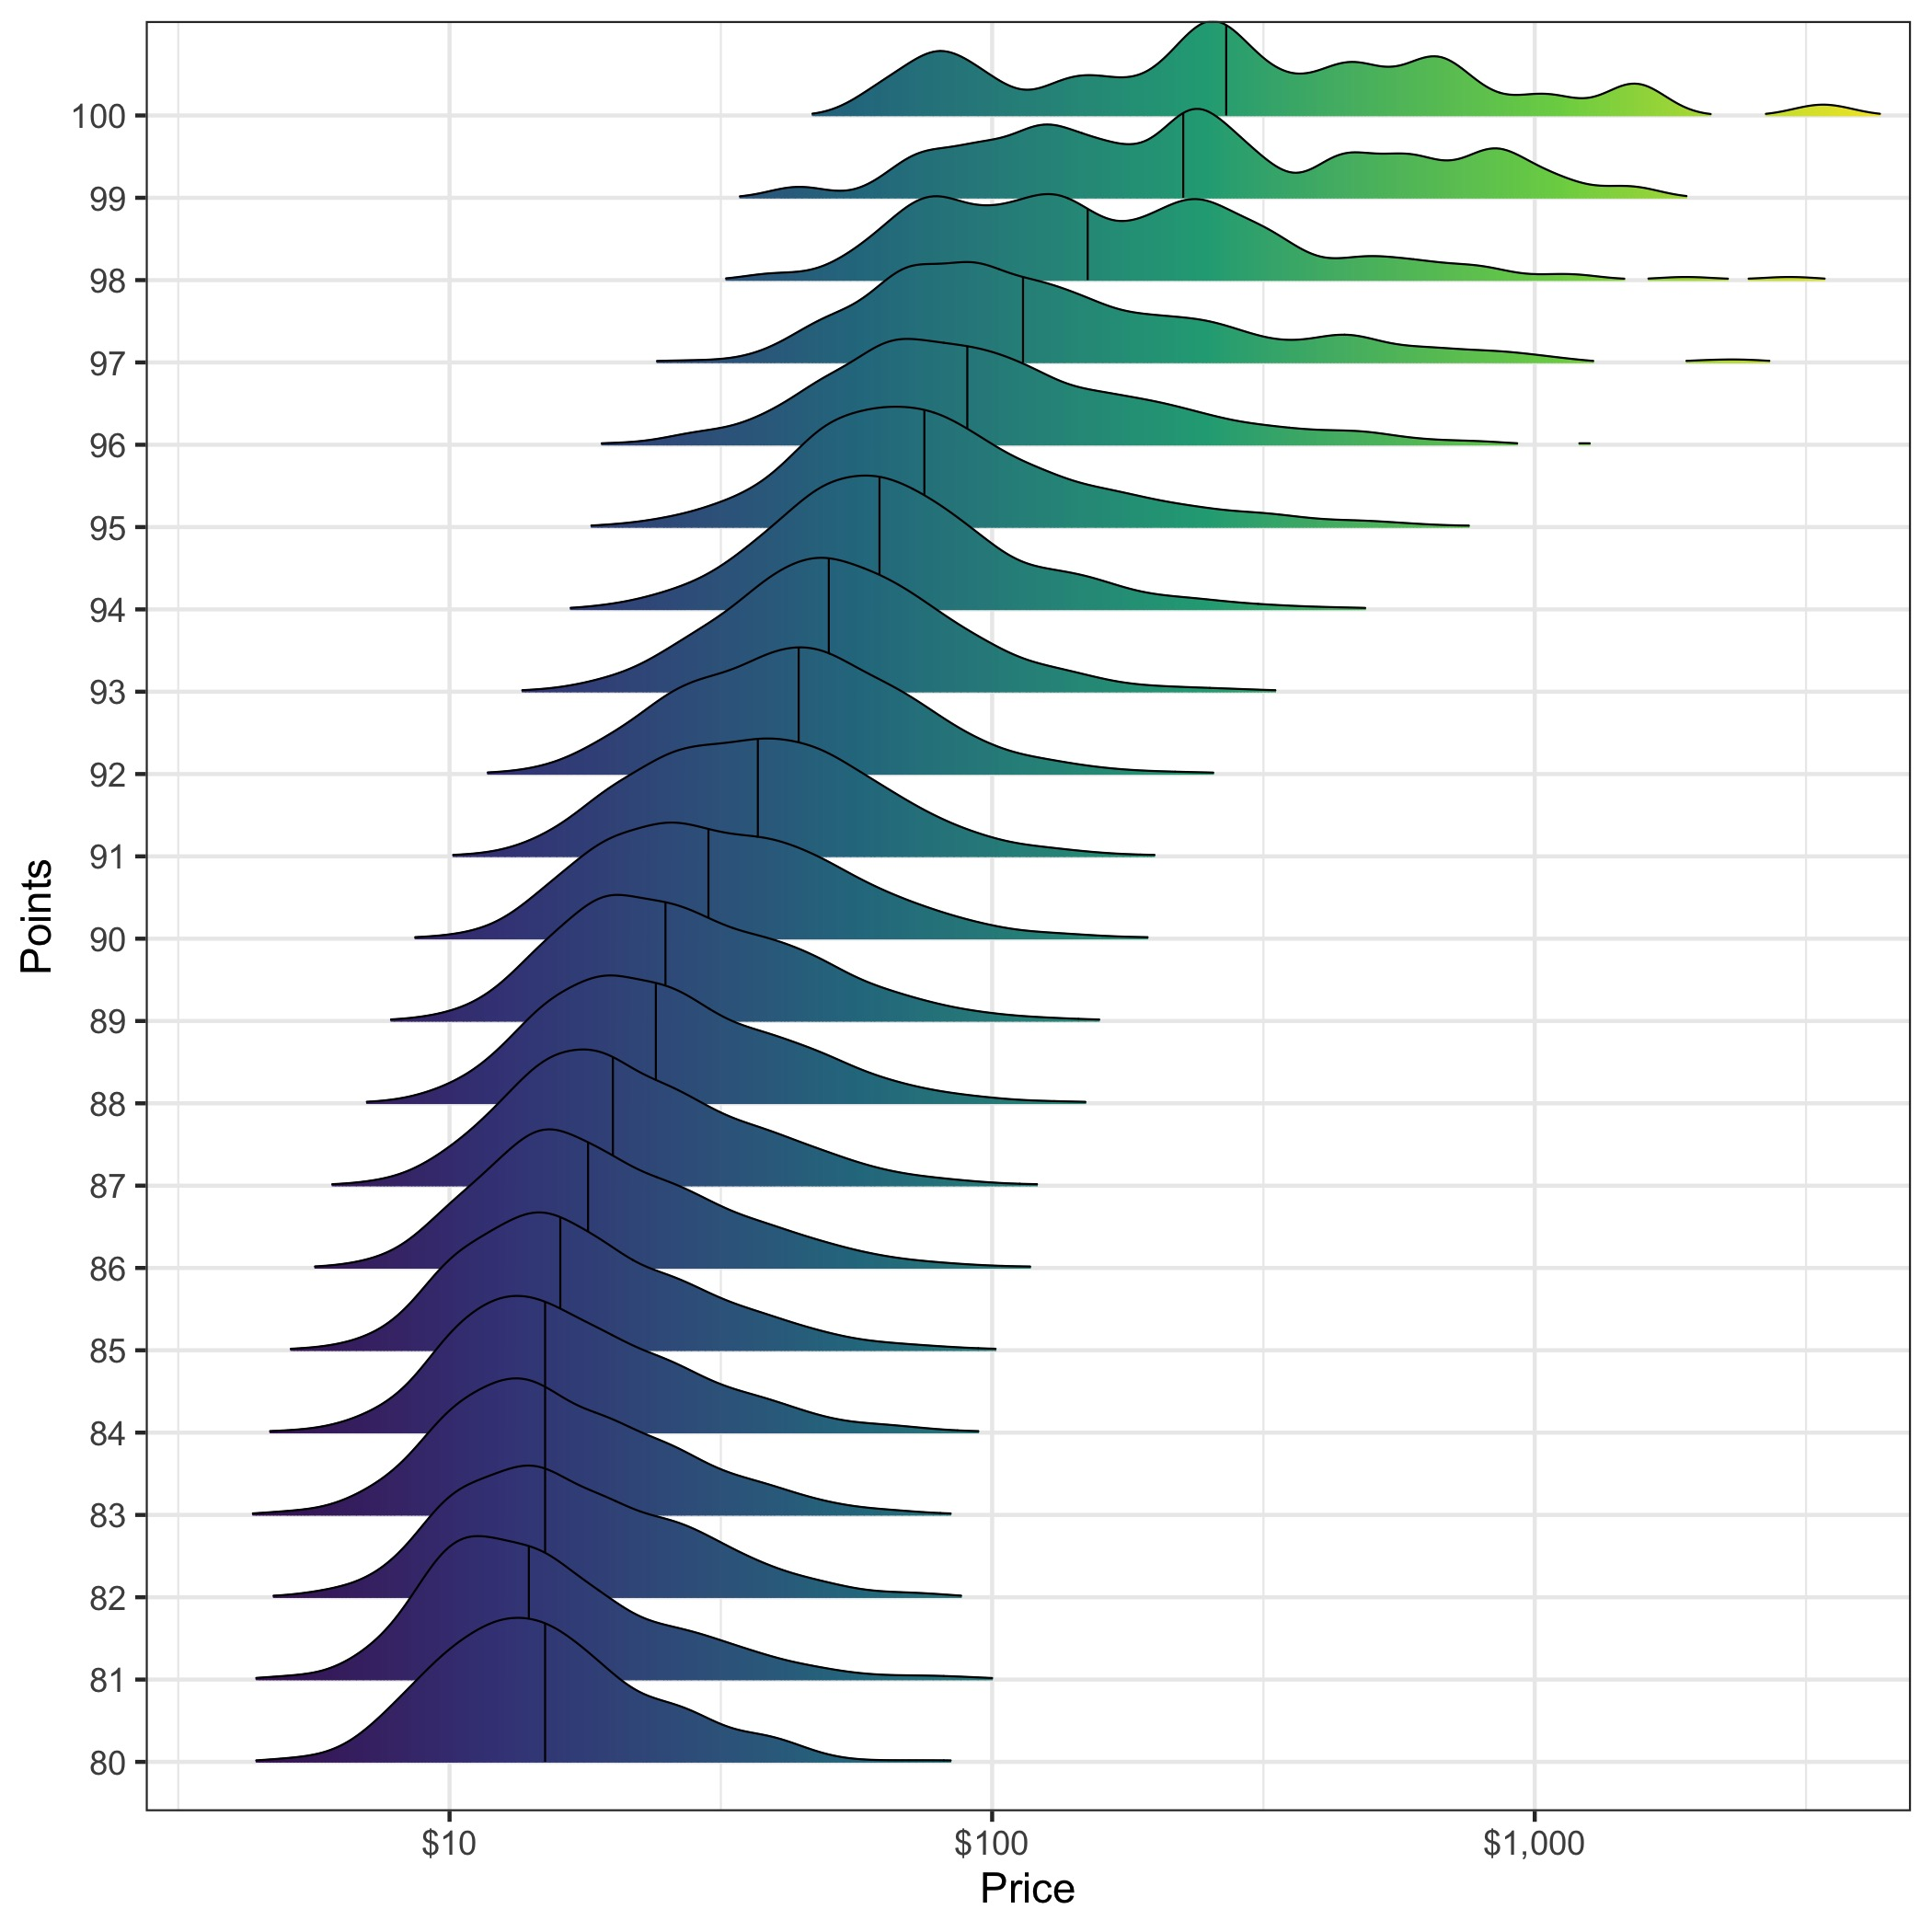
\includegraphics[width=0.95\linewidth]{3.jpg} 
  \caption{Mean and standard deviation of scoring by tasters} % Change caption
\end{figure}

As shown by figure 3, there is a clear difference in the scores given by the tasters. This however, doesn't necessarily indicate whether some tasters are nicer or harsher; it could simply be a case of certain tasters tasting inherently better wine and others tasting worse wine. There also doesn't seem to be a relationship between gender and scoring.

% 444444444
\subsection{Are pricier wines better?}
\emph{Wine Enthusiast} carries out a strict blind-tasting process that eliminates many possibilities for bias and ensures that the wines are scored only according to the characteristics of the liquids themselves \cite{WineMag}. It is especially important for the tasters to be unaware of the pricing because it has been shown that pricing influences how much humans like wine \cite{SchmidtSkvortsova2017}. In theory however, more expensive wine should indeed mean better quality, and thus, a more enjoyable and nicer taste. For the aforementioned reason, I decided to explore whether this is true in practice by visualizing the distribution of pricing across different points.

% Initially, scatter plots were tested

\begin{figure}[h]
  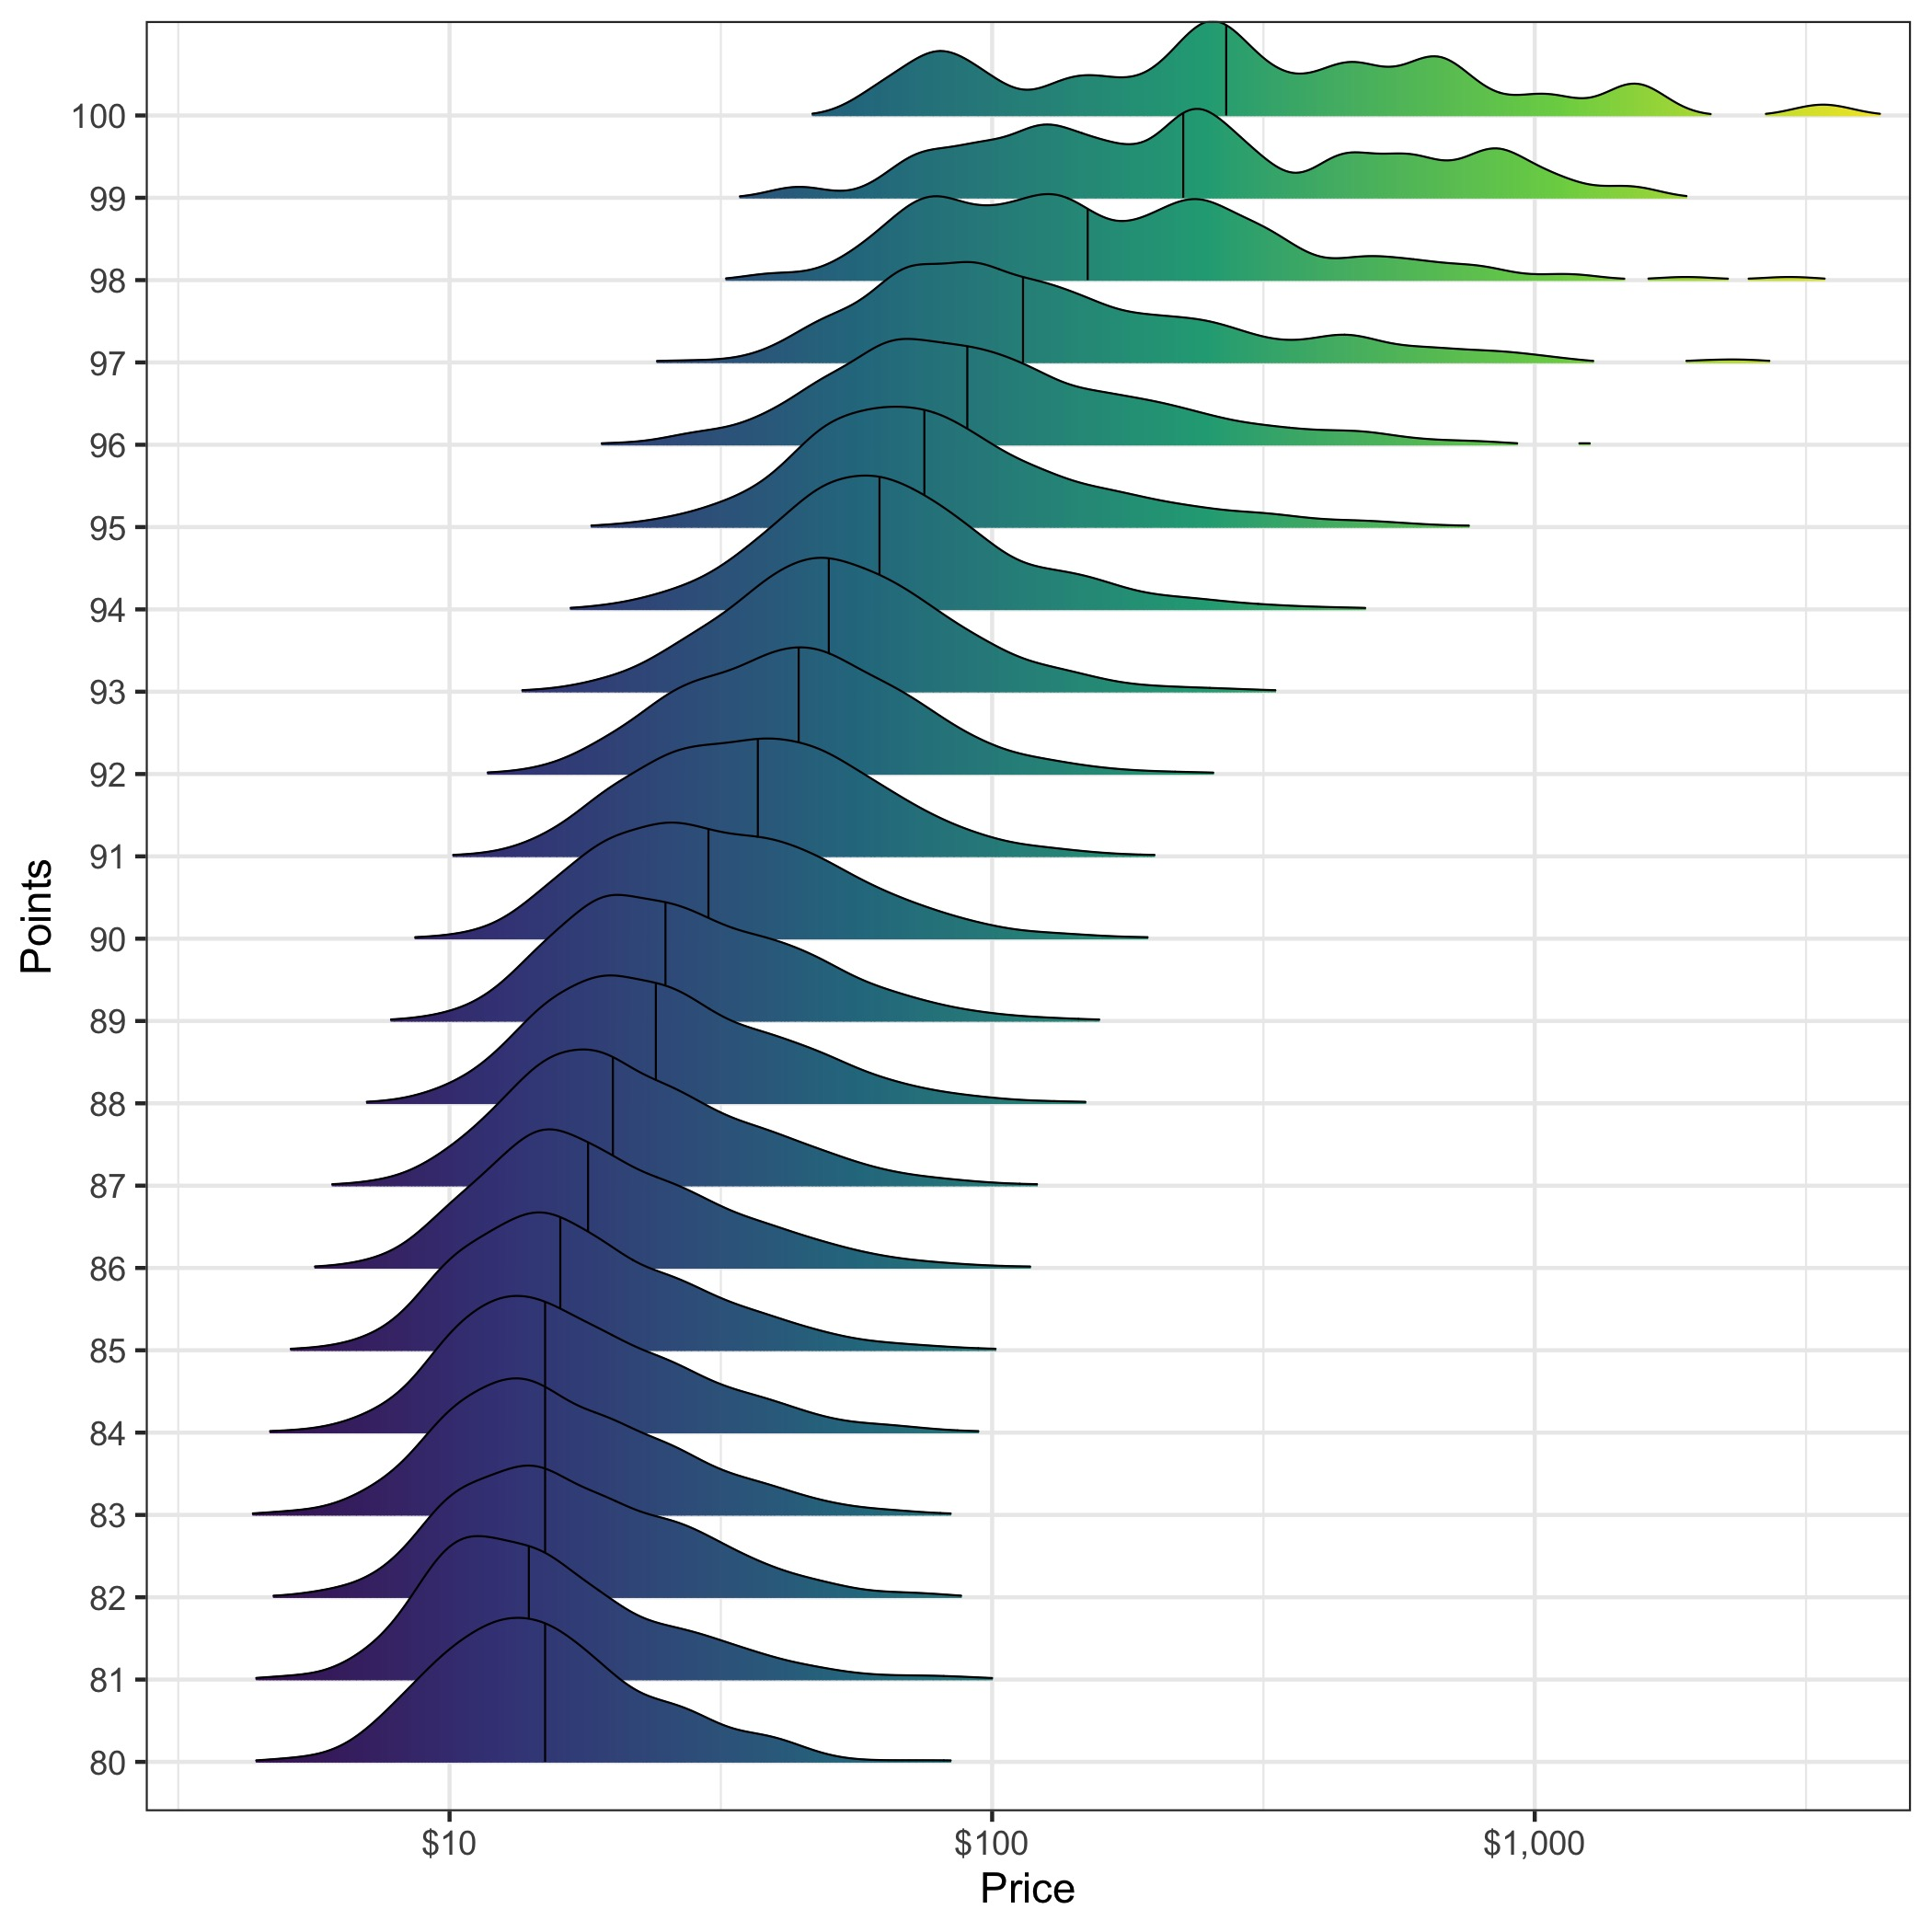
\includegraphics[width=0.95\linewidth]{4.jpg}
  \caption{Distribution of pricing for each points} % Change caption
\end{figure}

As shown by figure 4, pricier wines do indeed tend to taste better, though this trend does not become apparent until wines scoring 87 and above. However, as the score increases, the pricing distribution also becomes more spread out, which implicates that great wine can come at a wide range of prices.

The $x$-axis (which represents price) was logarithmically scaled because otherwise, the very wide range of prices would have lead to a very `zoomed out' plot that was hard to grasp information from. The median of each distribution was also added as a line to give a better idea of the trend. The gradient fill was added to help the viewers see increasing prices as the scores increased.

This figure follows the Gestalt principles of figure-ground, continuity, and closure to allow the viewer to easily interpret this visualization. The gradient fill and the black contour line of each distribution are contrasted with the white background so that the viewer can easily recognize the distributions. Additionally, the principles of continuity and closure allow the viewer to distinguish between the overlapping distributions.


\section{Further Exploration}

Upon completion of the visualizations meant to answer the initial research questions, further exploratory research questions were developed:

\begin{enumerate}
  \item Which wines have the best value in terms of the points to score ratio? 
  \item Do countries that produce wine consume more wine?
\end{enumerate}

\subsection{Which wines have the best value in terms of the price to points ratio (PPR)?}

To answer this question, multiple visualizations were made. One to compare how good the value of the wines produced by each country were, a second one to visualize the 10 wines with the best value, and third one to visualize the wines with scores above 90 with the best value.

\begin{figure}[h]
  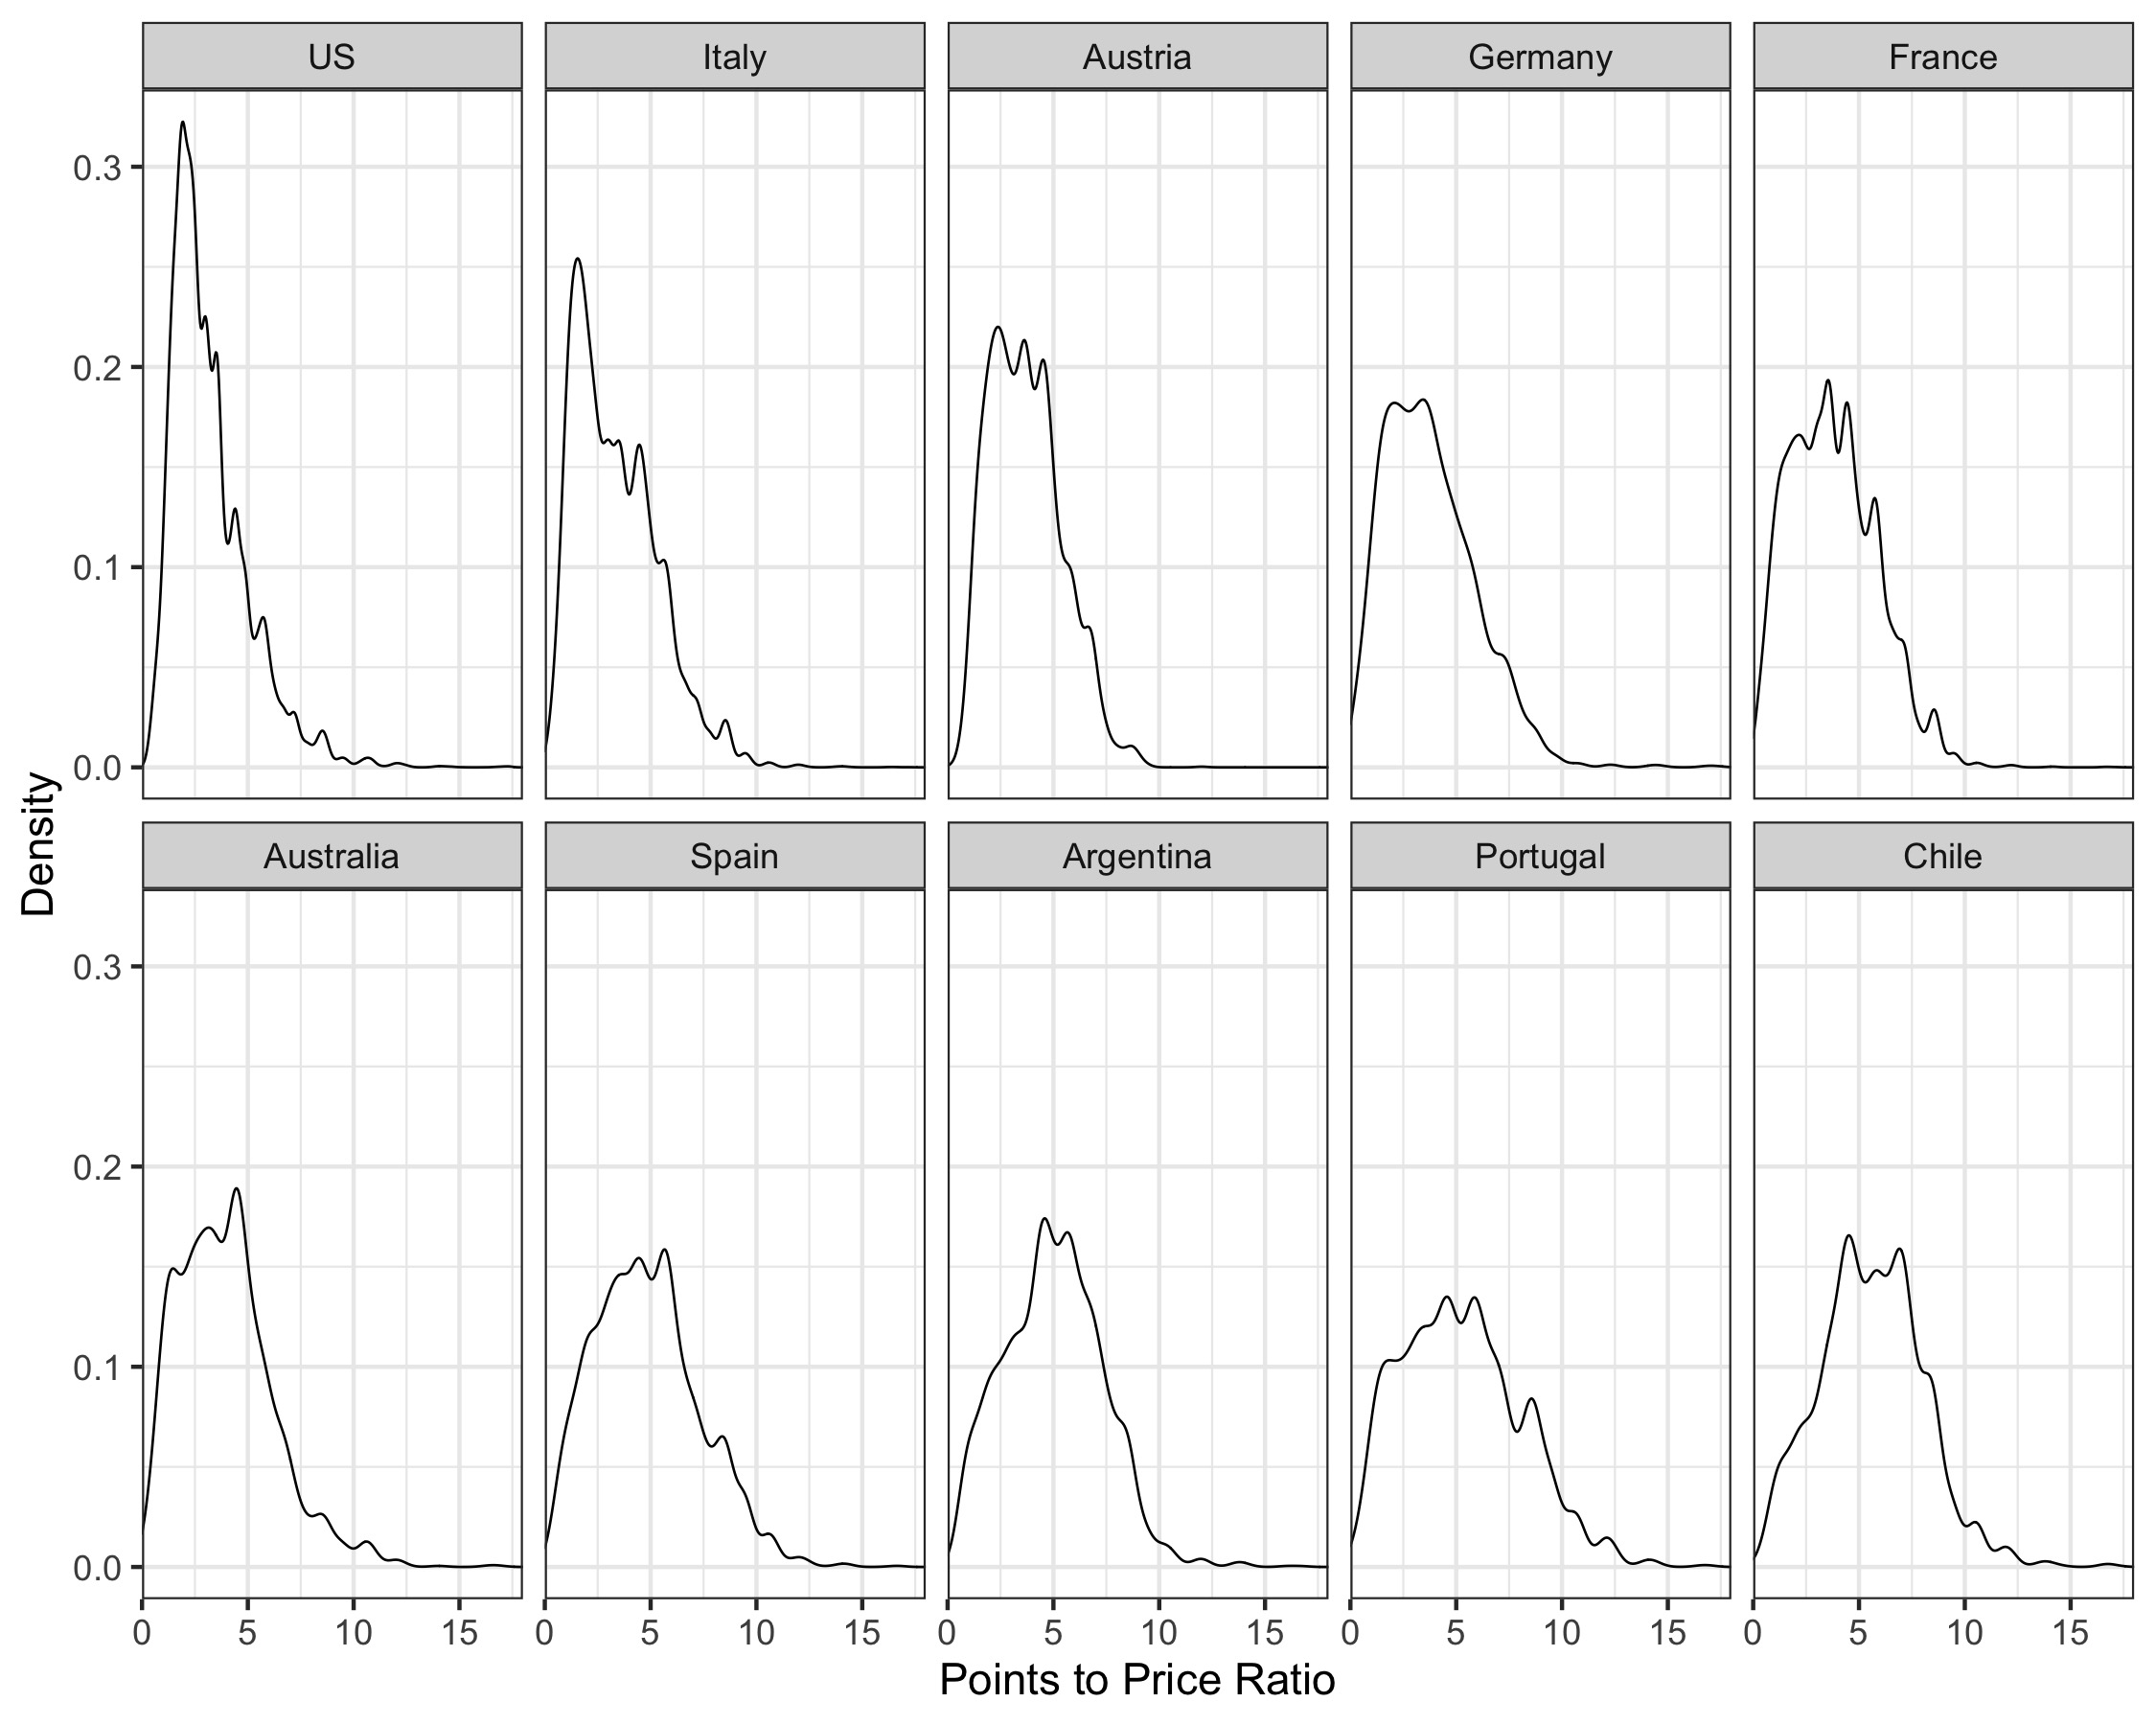
\includegraphics[width=0.95\linewidth]{5.1.jpg}
  \caption{PPR distributions of the wines produced by the 10 most reviewed countries} % Change caption
\end{figure}

Processing of the data involved dropping rows without a price, and creating a column for each wine's PPR by dividing their points by their price. Thus, the higher the PPR, the better the value.

A visualization of the distribution of each country's wine's PPR was first visualized using kernel density plots, which were faceted for more clarity. The facets are displayed in ascending order of each country's mean PPR as opposed to the default alphabetical order to better see the differences in distribution; this was accomplished by first grouping the data by country, calculating the mean PPR of each country, sorting it in ascending order, and extracting this ordered list of countries as a vector to use to override \code{facet\_wrap()}'s alphabetical ordering. Additionally, only the 10 most reviewed countries were considered because of reasons related to the sample size and the fact that there is a large amount of countries.

As shown by figure 5, all countries have a similar underlying distribution, however, it is clear that a large percentage of wines reviewed from the US and Italy have poor value compared to the other countries.

The second visualization shows the 10 wines with the highest PPR. For the previously mentioned reasons, a Cleveland dot plot was used again. As shown by figure 6, the best valued wines are all scored between 86 and 83, which perfectly falls into \emph{Wine Enthusiast's} classification of \emph{good} wine---`[s]uitable for everyday consumption; often good value' \cite{WineMag}---and, interestingly, all of the wines in figure 6 cost 4 dollars. Because there were no wines scored above 94 (\emph{superb} and beyond as classified by \emph{Wine Enthusiast}), another plot was made to see which wines scoring 94 points or had the best value.

\begin{figure}[h]
  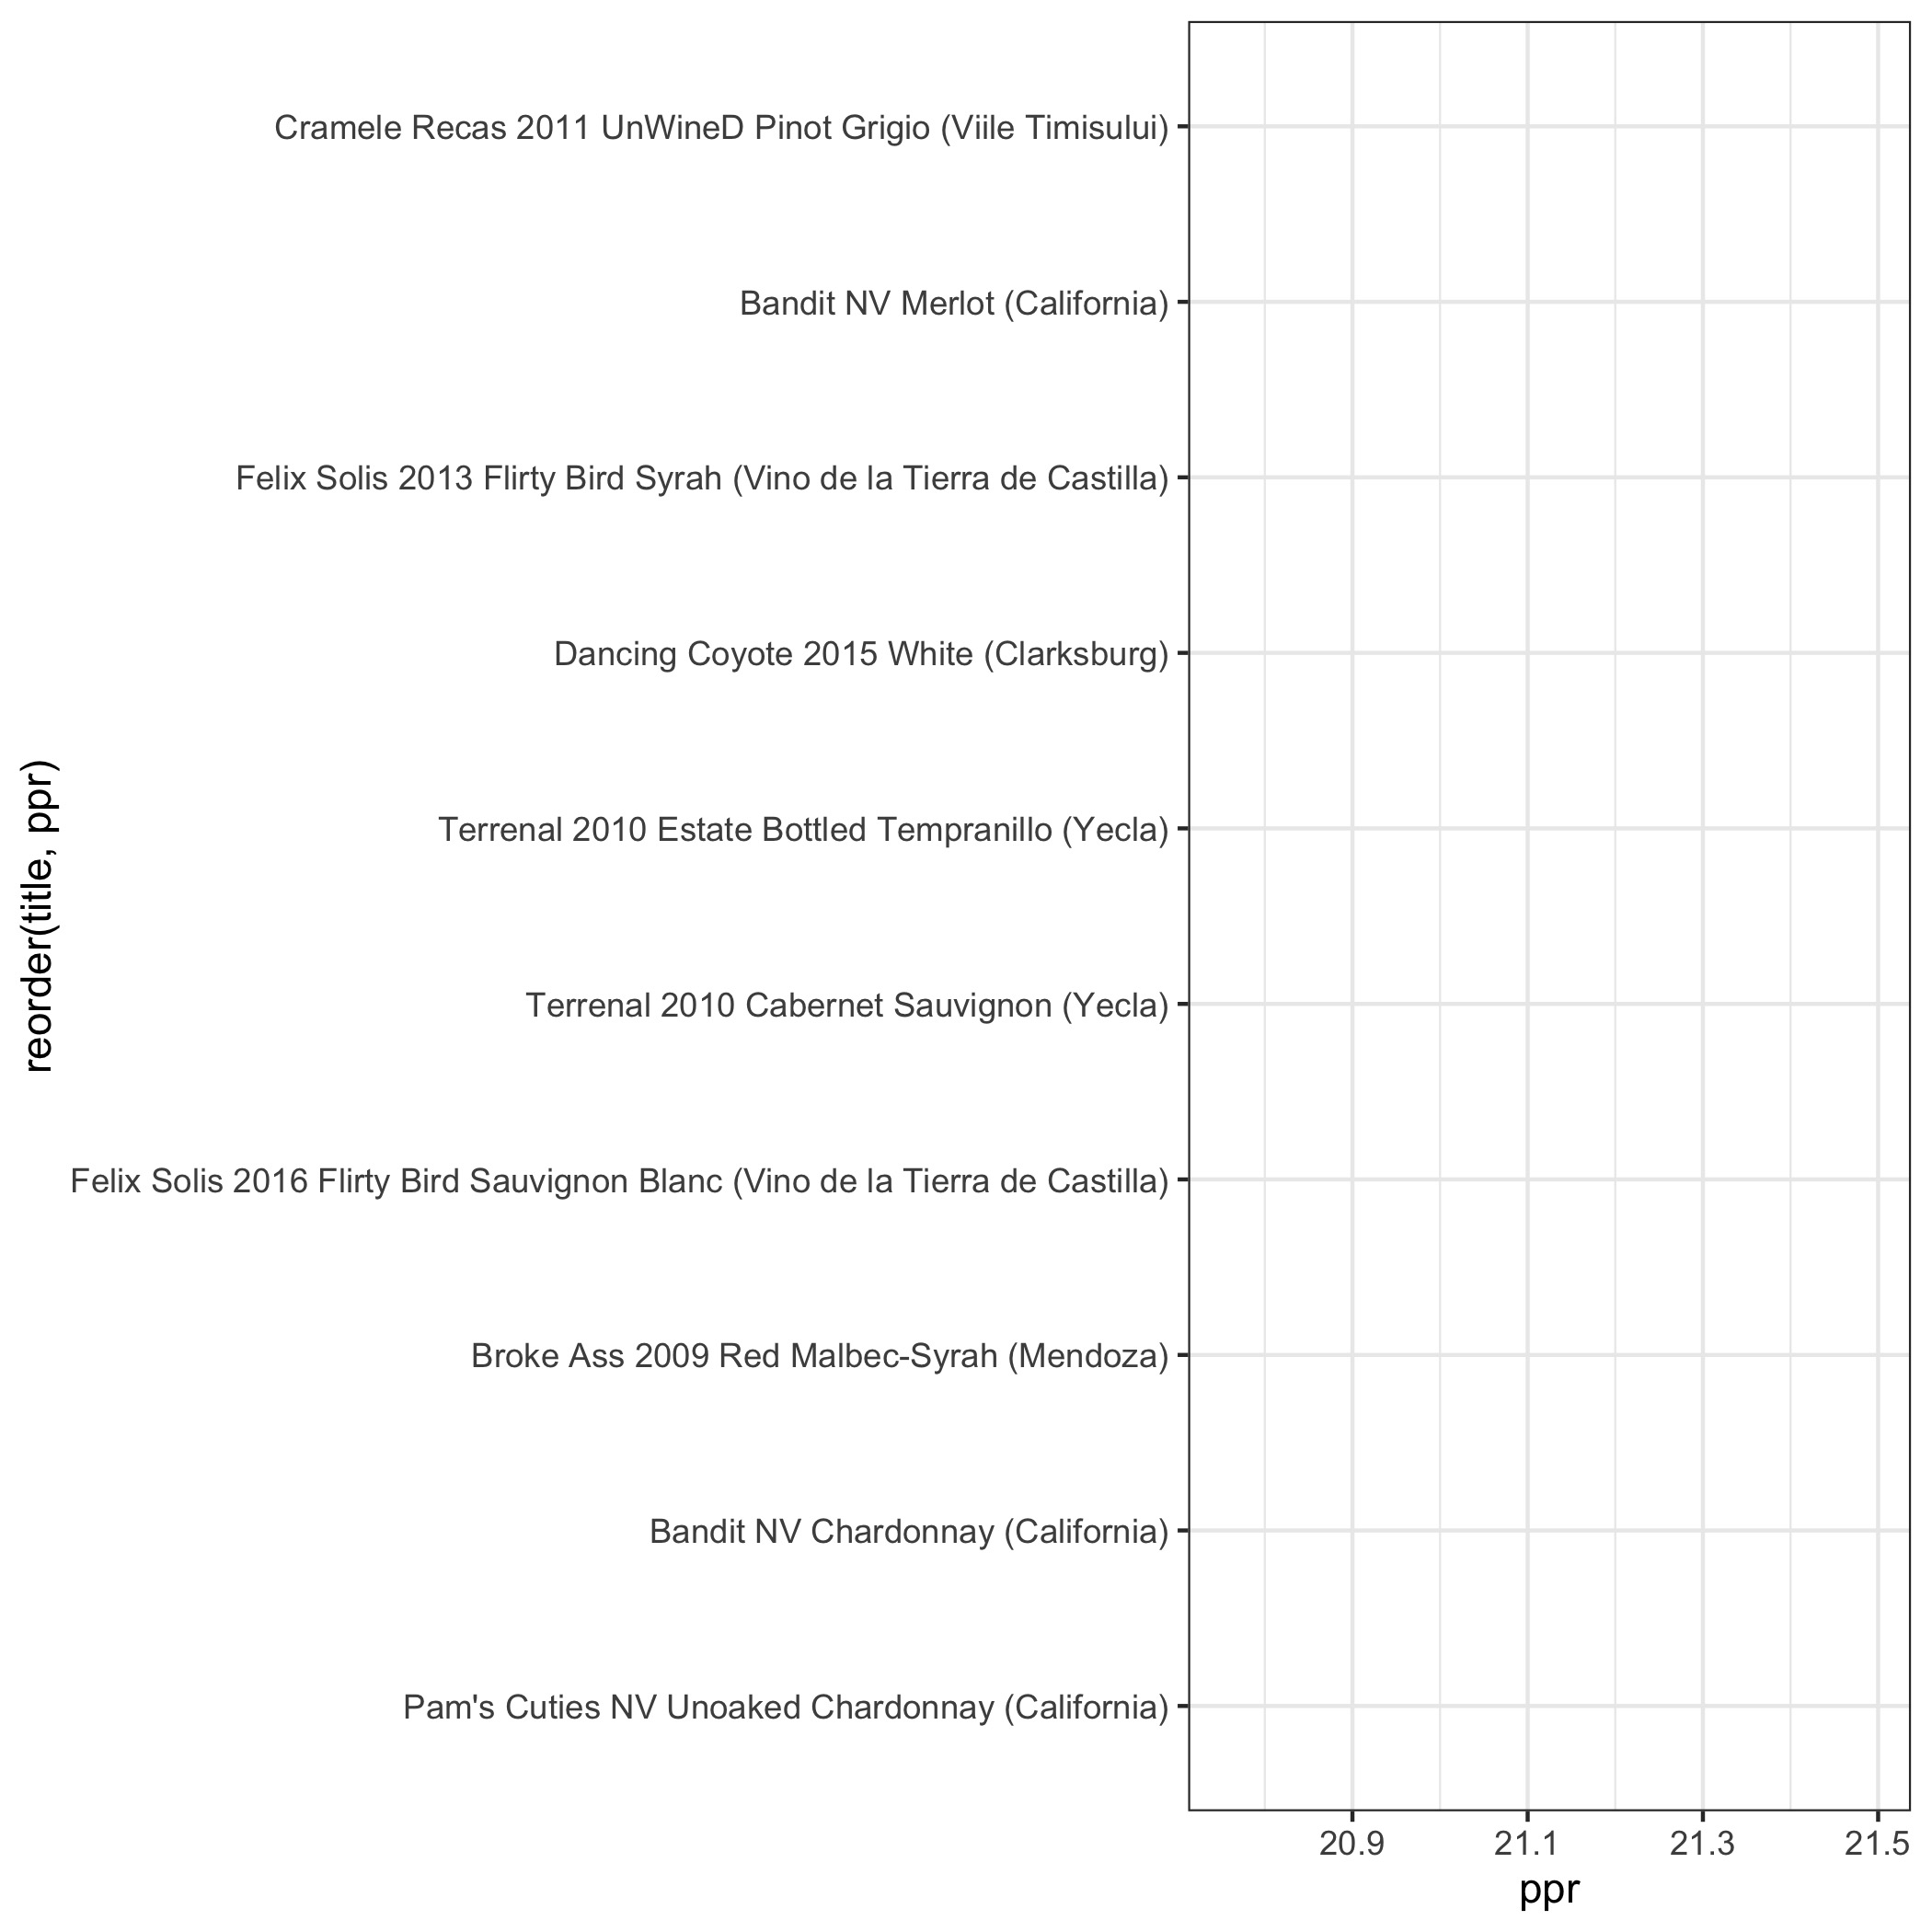
\includegraphics[width=0.95\linewidth]{5.2.jpg}
  \caption{Wines by PPR}
\end{figure}

\begin{figure}[h]
  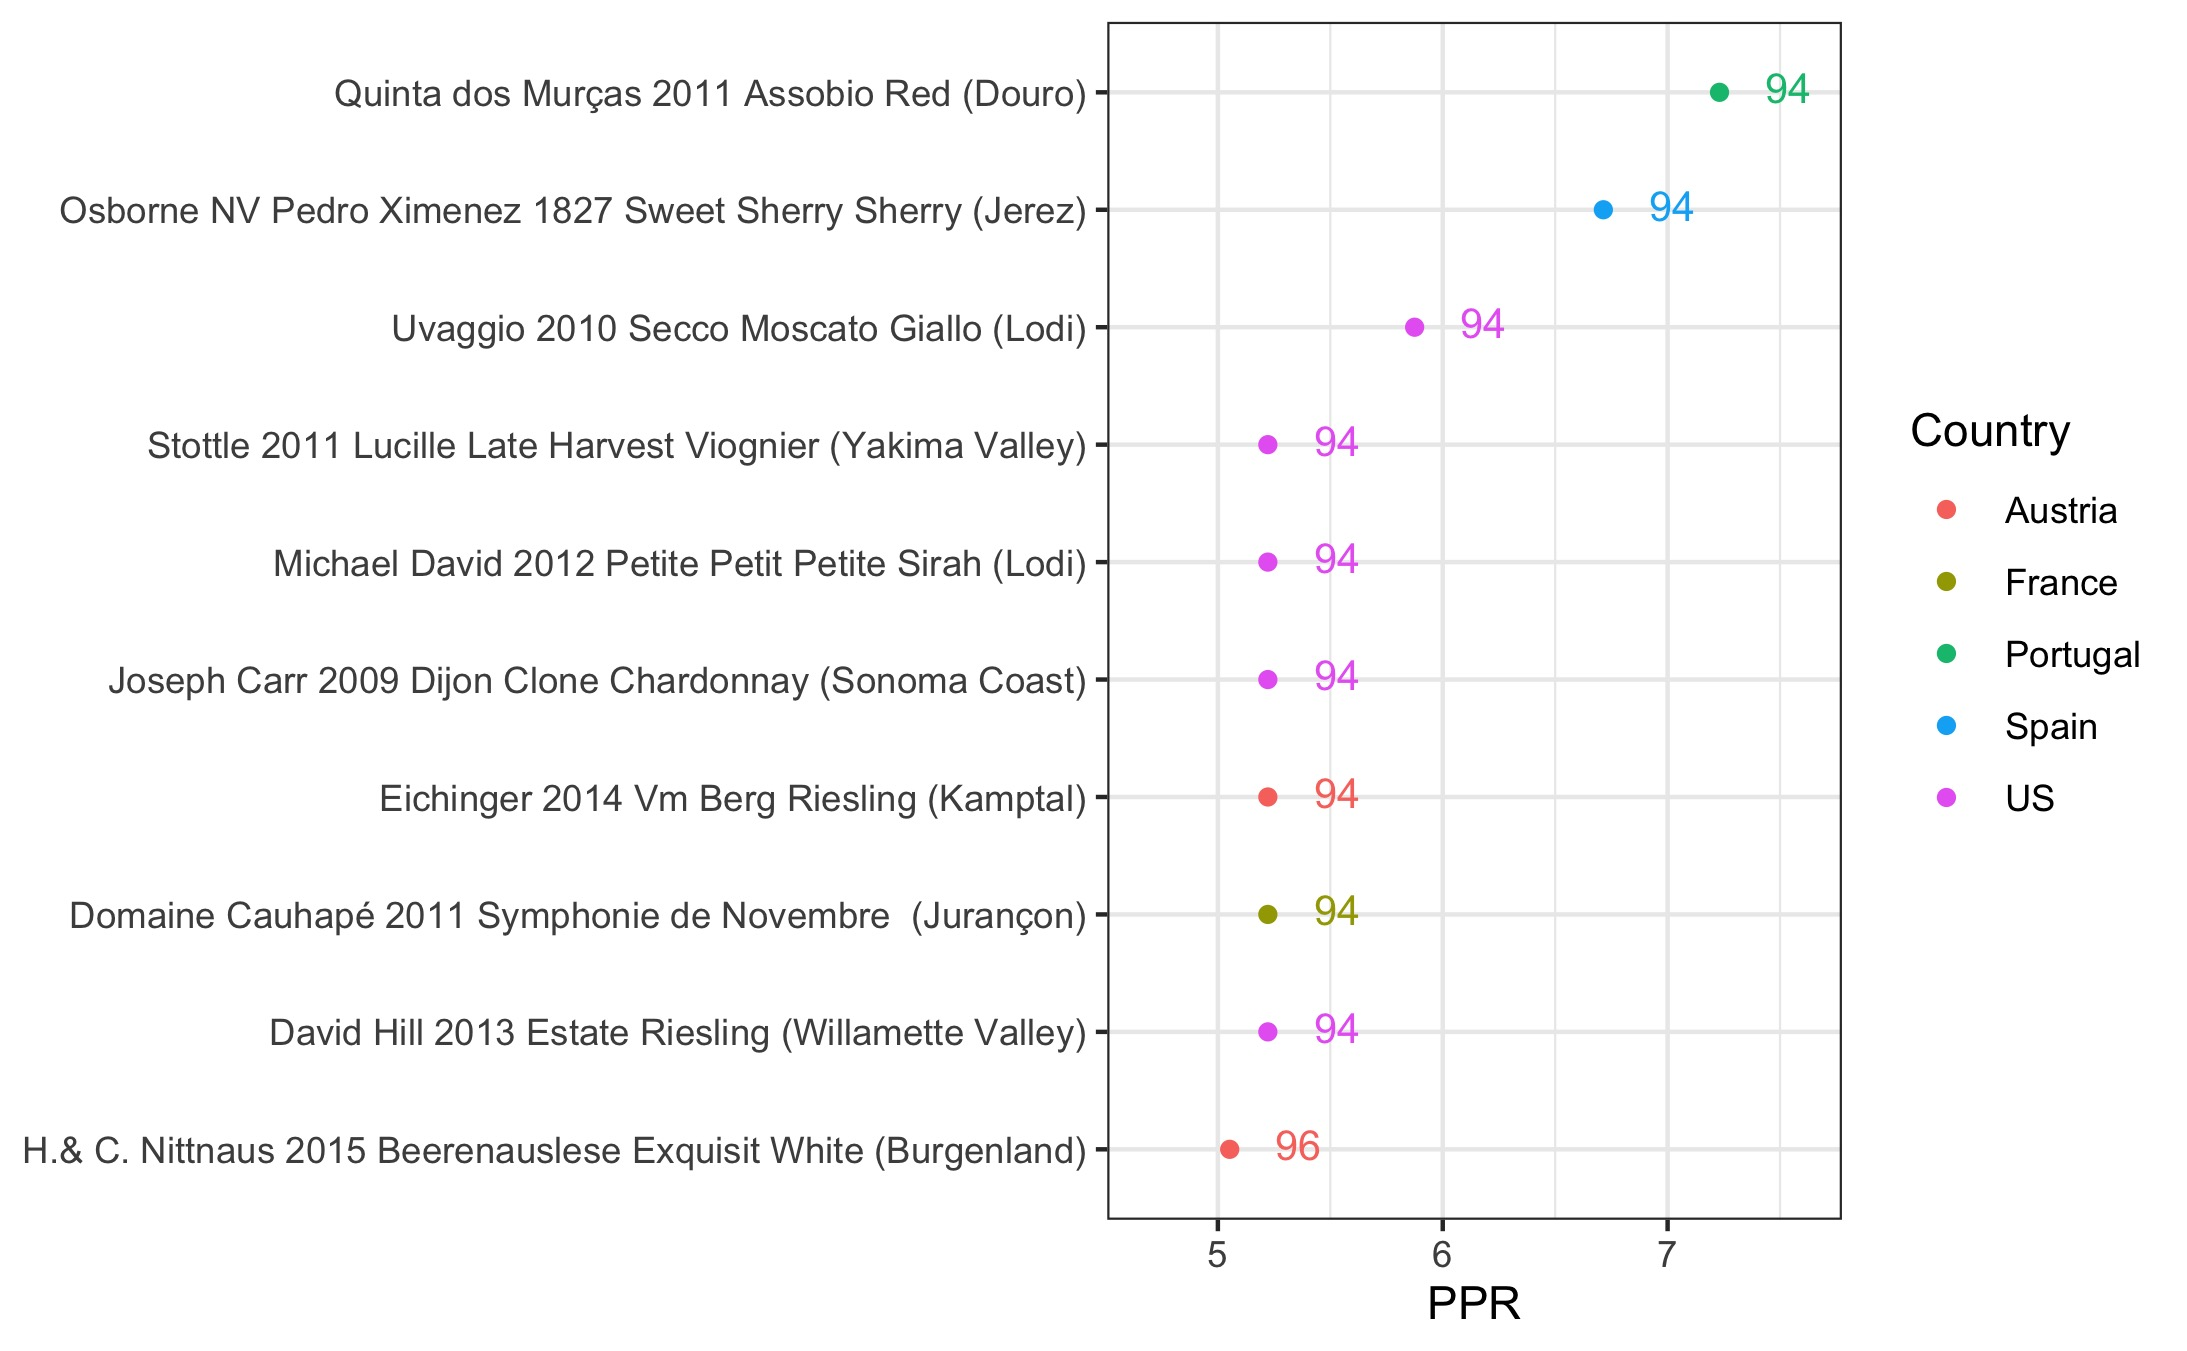
\includegraphics[width=0.95\linewidth]{5.3.jpg}
  \caption{Wines scoring more than 94 by PPR}
\end{figure}

\subsection{Does wine consumption increase with wine production?}

The final question aims to explore whether countries that produce wine consume more of it compared to countries that produce less. The data required to answer this question isn't present in the original datasets so the wine consumption and production data in 2016 was gathered from the \emph{International Organisation of Vine and Wine} \cite{OIV}. While the values for consumption were already presented as liters per capita, the values for production were in 1000 hectoliters. To standardize the value to liters produced per capita, population data was obtained from \emph{The World Bank} database \cite{WorldBank}.

To produce the required data, the tables for consumption, production, and population were joined by country. A new column for the wine production in liters per capita was created by multiplying the original production values by 1000 and 100 (1 hectoliter = 100 liters), and diving the previous result by the population.

The scatter plot was used because they are particularly effective for observing relationships between two quantitative variables, which is supported by the fact that position is the most effective at encoding quantitative values \cite{Mackinlay}. Color is used to encode the continents alongside a reduced opacity for each point to better distinguish them, especially the ones that are clustered near the origin. A smoothing line was fit to the graph using a generalized additive model to better see the relationship between the two variables.

\begin{figure}[h]
  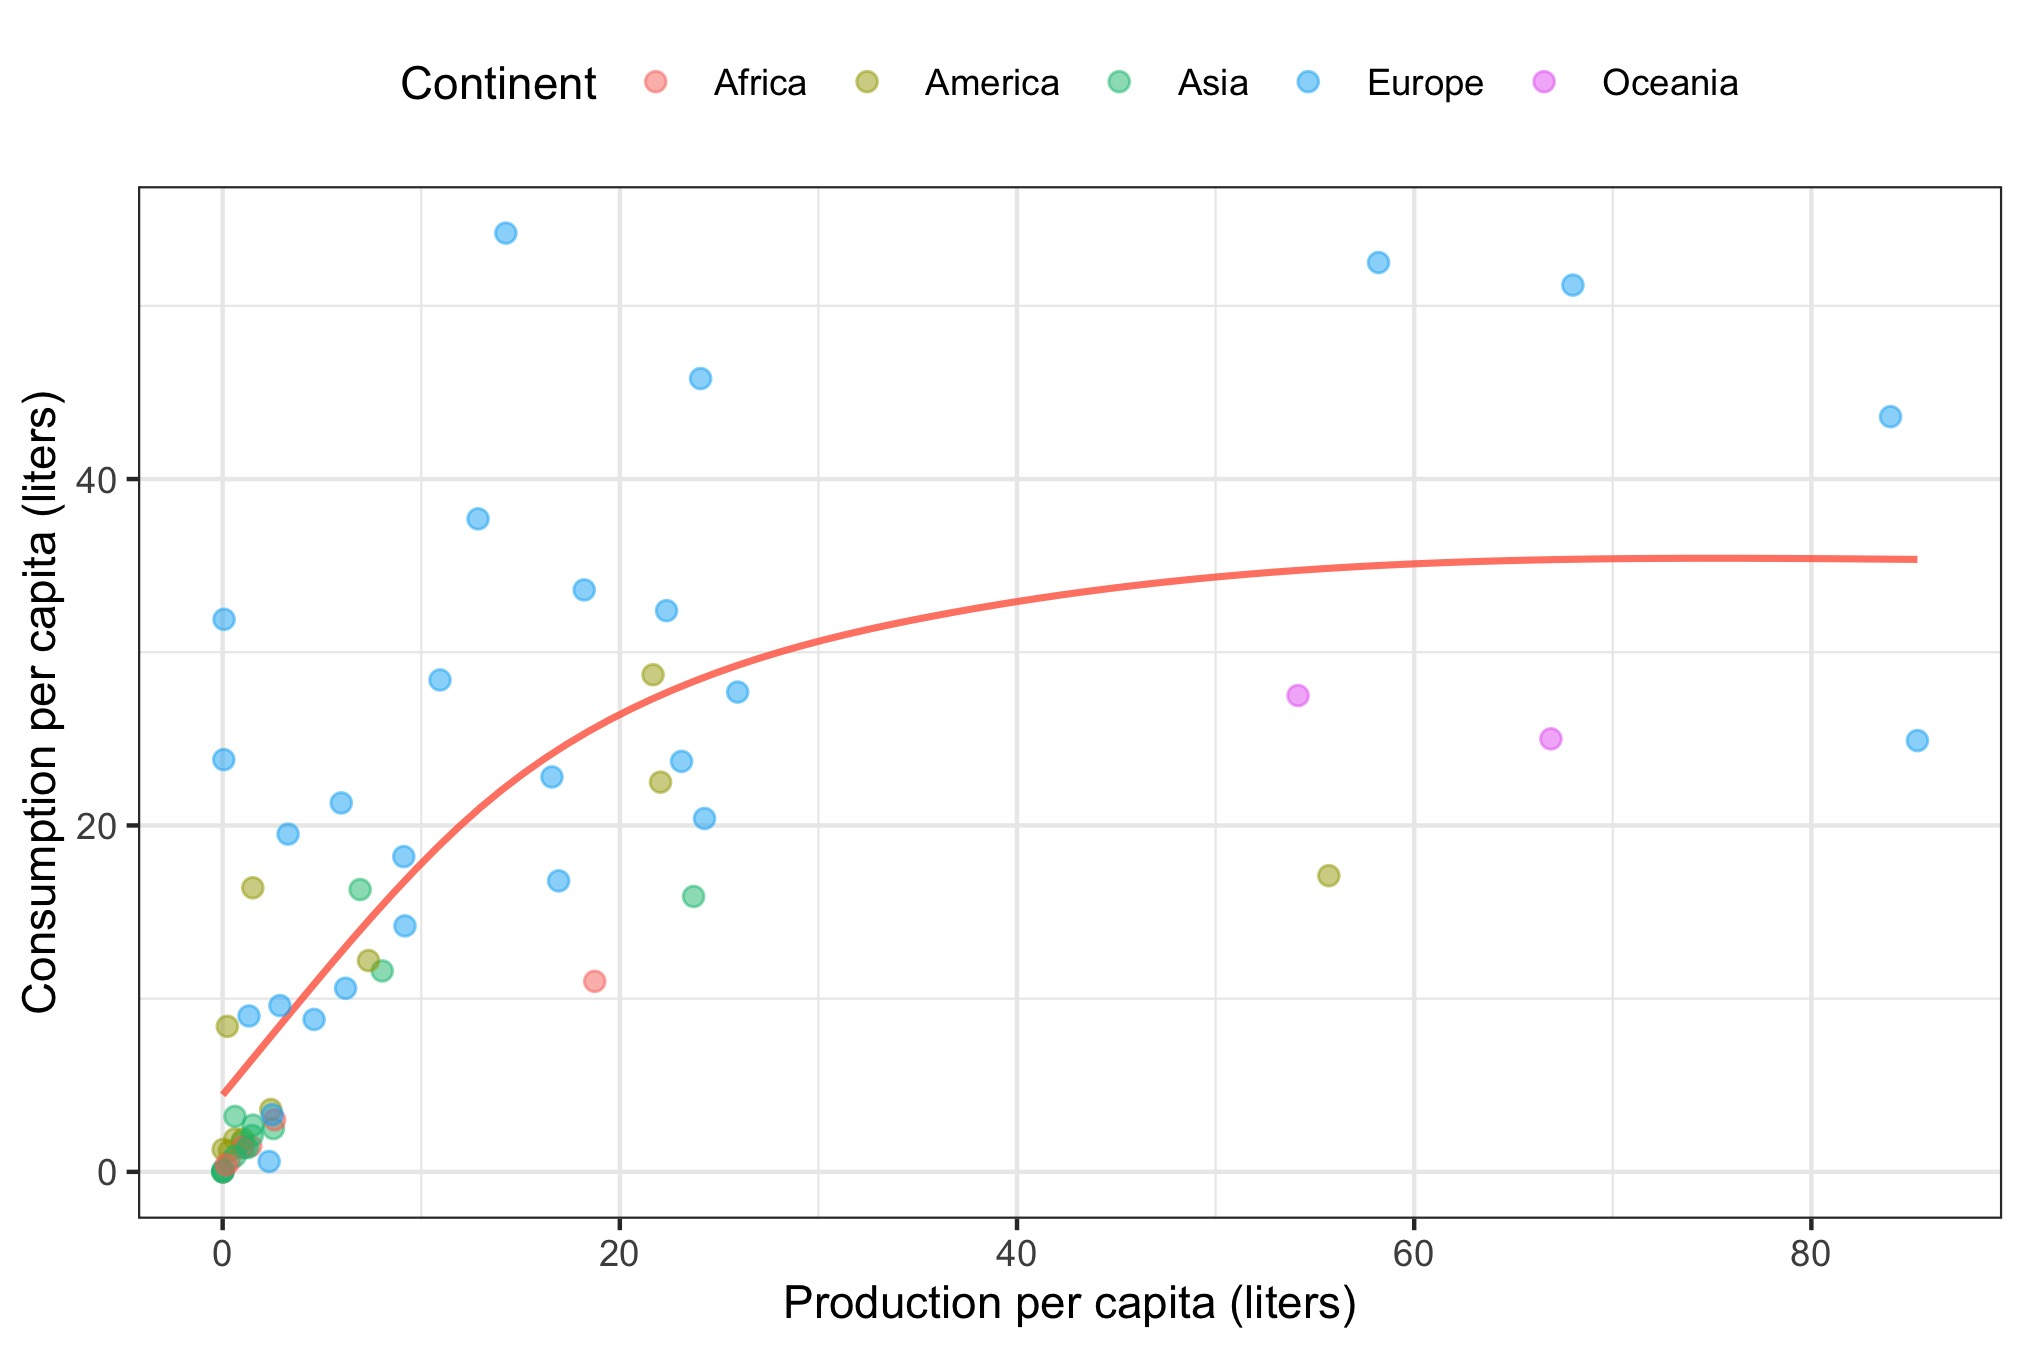
\includegraphics[width=0.95\linewidth]{6.jpg}
  \caption{Wine production vs. wine consumption}
\end{figure}

As shown by figure 6, there seems to be a positive relationship between consumption and production until it begins to flatten, such that after a production of 30 liters per capita, further increases do not necessarily lead to a higher consumption. However, there is significantly less data for countries with a production value of more than 30 liters per capita; while the three European countries above the line support the hypothesis that a higher wine production leads to more consumption, the four countries below the line contradict it, thus, more data is required to reach a conclusion.


\section{Exploratory Process and Reflection}

Because the dataset was the starting point of this work (rather than a set of questions or points to be proven), the initial questions were generated by considering the variables available in the dataset, and trying to understand what is interesting about it through exploratory data analysis. Answering the questions was simply a matter of transforming the raw data into tables that are ready to be visually mapped, and then creating the visualizations themselves. Then, Through an iterative trial and error process, different types of plots and encodings were tested, all with the goal of producing expressive and effective visualizations. After selecting a visual encoding, small details were refined to make the plot more appealing and simple while being able to convey the main ideas of the visualization. The process followed was essentially the seven stages of visualization outlined by Ben Fry in his work \emph{Visualizing Data}---acquire, parse, filter, mine, represent, and refine---except for addition of interaction \cite{Fry}.

The first further exploratory question were formed after analyzing the results of the fourth initial question; seeing the visualization made me understand that good wine doesn't necessarily have to be very expensive like I previously thought, so I really wanted to know what wines gave the best bang for your buck. The second further exploratory question was developed after learning from research for the first initial question that Italy, France, and Spain produce a lot more wine than the US even though they are much smaller.

Overall, even though I had no prior knowledge of wines and its markets, I found the whole process very enjoyable, from uncovering interesting relationships and information, and producing effective and appealing visualizations.
    
\printbibliography